% Options for packages loaded elsewhere
% Options for packages loaded elsewhere
\PassOptionsToPackage{unicode}{hyperref}
\PassOptionsToPackage{hyphens}{url}
\PassOptionsToPackage{dvipsnames,svgnames,x11names}{xcolor}
%
\documentclass[
  spanish,
  11pt,
  a4paper,
  DIV=11,
  numbers=noendperiod]{scrartcl}
\usepackage{xcolor}
\usepackage[margin=2.5cm]{geometry}
\usepackage{amsmath,amssymb}
\setcounter{secnumdepth}{5}
\usepackage{iftex}
\ifPDFTeX
  \usepackage[T1]{fontenc}
  \usepackage[utf8]{inputenc}
  \usepackage{textcomp} % provide euro and other symbols
\else % if luatex or xetex
  \usepackage{unicode-math} % this also loads fontspec
  \defaultfontfeatures{Scale=MatchLowercase}
  \defaultfontfeatures[\rmfamily]{Ligatures=TeX,Scale=1}
\fi
\usepackage{lmodern}
\ifPDFTeX\else
  % xetex/luatex font selection
\fi
% Use upquote if available, for straight quotes in verbatim environments
\IfFileExists{upquote.sty}{\usepackage{upquote}}{}
\IfFileExists{microtype.sty}{% use microtype if available
  \usepackage[]{microtype}
  \UseMicrotypeSet[protrusion]{basicmath} % disable protrusion for tt fonts
}{}
\makeatletter
\@ifundefined{KOMAClassName}{% if non-KOMA class
  \IfFileExists{parskip.sty}{%
    \usepackage{parskip}
  }{% else
    \setlength{\parindent}{0pt}
    \setlength{\parskip}{6pt plus 2pt minus 1pt}}
}{% if KOMA class
  \KOMAoptions{parskip=half}}
\makeatother
% Make \paragraph and \subparagraph free-standing
\makeatletter
\ifx\paragraph\undefined\else
  \let\oldparagraph\paragraph
  \renewcommand{\paragraph}{
    \@ifstar
      \xxxParagraphStar
      \xxxParagraphNoStar
  }
  \newcommand{\xxxParagraphStar}[1]{\oldparagraph*{#1}\mbox{}}
  \newcommand{\xxxParagraphNoStar}[1]{\oldparagraph{#1}\mbox{}}
\fi
\ifx\subparagraph\undefined\else
  \let\oldsubparagraph\subparagraph
  \renewcommand{\subparagraph}{
    \@ifstar
      \xxxSubParagraphStar
      \xxxSubParagraphNoStar
  }
  \newcommand{\xxxSubParagraphStar}[1]{\oldsubparagraph*{#1}\mbox{}}
  \newcommand{\xxxSubParagraphNoStar}[1]{\oldsubparagraph{#1}\mbox{}}
\fi
\makeatother

\usepackage{color}
\usepackage{fancyvrb}
\newcommand{\VerbBar}{|}
\newcommand{\VERB}{\Verb[commandchars=\\\{\}]}
\DefineVerbatimEnvironment{Highlighting}{Verbatim}{commandchars=\\\{\}}
% Add ',fontsize=\small' for more characters per line
\usepackage{framed}
\definecolor{shadecolor}{RGB}{241,243,245}
\newenvironment{Shaded}{\begin{snugshade}}{\end{snugshade}}
\newcommand{\AlertTok}[1]{\textcolor[rgb]{0.68,0.00,0.00}{#1}}
\newcommand{\AnnotationTok}[1]{\textcolor[rgb]{0.37,0.37,0.37}{#1}}
\newcommand{\AttributeTok}[1]{\textcolor[rgb]{0.40,0.45,0.13}{#1}}
\newcommand{\BaseNTok}[1]{\textcolor[rgb]{0.68,0.00,0.00}{#1}}
\newcommand{\BuiltInTok}[1]{\textcolor[rgb]{0.00,0.23,0.31}{#1}}
\newcommand{\CharTok}[1]{\textcolor[rgb]{0.13,0.47,0.30}{#1}}
\newcommand{\CommentTok}[1]{\textcolor[rgb]{0.37,0.37,0.37}{#1}}
\newcommand{\CommentVarTok}[1]{\textcolor[rgb]{0.37,0.37,0.37}{\textit{#1}}}
\newcommand{\ConstantTok}[1]{\textcolor[rgb]{0.56,0.35,0.01}{#1}}
\newcommand{\ControlFlowTok}[1]{\textcolor[rgb]{0.00,0.23,0.31}{\textbf{#1}}}
\newcommand{\DataTypeTok}[1]{\textcolor[rgb]{0.68,0.00,0.00}{#1}}
\newcommand{\DecValTok}[1]{\textcolor[rgb]{0.68,0.00,0.00}{#1}}
\newcommand{\DocumentationTok}[1]{\textcolor[rgb]{0.37,0.37,0.37}{\textit{#1}}}
\newcommand{\ErrorTok}[1]{\textcolor[rgb]{0.68,0.00,0.00}{#1}}
\newcommand{\ExtensionTok}[1]{\textcolor[rgb]{0.00,0.23,0.31}{#1}}
\newcommand{\FloatTok}[1]{\textcolor[rgb]{0.68,0.00,0.00}{#1}}
\newcommand{\FunctionTok}[1]{\textcolor[rgb]{0.28,0.35,0.67}{#1}}
\newcommand{\ImportTok}[1]{\textcolor[rgb]{0.00,0.46,0.62}{#1}}
\newcommand{\InformationTok}[1]{\textcolor[rgb]{0.37,0.37,0.37}{#1}}
\newcommand{\KeywordTok}[1]{\textcolor[rgb]{0.00,0.23,0.31}{\textbf{#1}}}
\newcommand{\NormalTok}[1]{\textcolor[rgb]{0.00,0.23,0.31}{#1}}
\newcommand{\OperatorTok}[1]{\textcolor[rgb]{0.37,0.37,0.37}{#1}}
\newcommand{\OtherTok}[1]{\textcolor[rgb]{0.00,0.23,0.31}{#1}}
\newcommand{\PreprocessorTok}[1]{\textcolor[rgb]{0.68,0.00,0.00}{#1}}
\newcommand{\RegionMarkerTok}[1]{\textcolor[rgb]{0.00,0.23,0.31}{#1}}
\newcommand{\SpecialCharTok}[1]{\textcolor[rgb]{0.37,0.37,0.37}{#1}}
\newcommand{\SpecialStringTok}[1]{\textcolor[rgb]{0.13,0.47,0.30}{#1}}
\newcommand{\StringTok}[1]{\textcolor[rgb]{0.13,0.47,0.30}{#1}}
\newcommand{\VariableTok}[1]{\textcolor[rgb]{0.07,0.07,0.07}{#1}}
\newcommand{\VerbatimStringTok}[1]{\textcolor[rgb]{0.13,0.47,0.30}{#1}}
\newcommand{\WarningTok}[1]{\textcolor[rgb]{0.37,0.37,0.37}{\textit{#1}}}

\usepackage{longtable,booktabs,array}
\usepackage{calc} % for calculating minipage widths
% Correct order of tables after \paragraph or \subparagraph
\usepackage{etoolbox}
\makeatletter
\patchcmd\longtable{\par}{\if@noskipsec\mbox{}\fi\par}{}{}
\makeatother
% Allow footnotes in longtable head/foot
\IfFileExists{footnotehyper.sty}{\usepackage{footnotehyper}}{\usepackage{footnote}}
\makesavenoteenv{longtable}
\usepackage{graphicx}
\makeatletter
\newsavebox\pandoc@box
\newcommand*\pandocbounded[1]{% scales image to fit in text height/width
  \sbox\pandoc@box{#1}%
  \Gscale@div\@tempa{\textheight}{\dimexpr\ht\pandoc@box+\dp\pandoc@box\relax}%
  \Gscale@div\@tempb{\linewidth}{\wd\pandoc@box}%
  \ifdim\@tempb\p@<\@tempa\p@\let\@tempa\@tempb\fi% select the smaller of both
  \ifdim\@tempa\p@<\p@\scalebox{\@tempa}{\usebox\pandoc@box}%
  \else\usebox{\pandoc@box}%
  \fi%
}
% Set default figure placement to htbp
\def\fps@figure{htbp}
\makeatother



\ifLuaTeX
\usepackage[bidi=basic]{babel}
\else
\usepackage[bidi=default]{babel}
\fi
% get rid of language-specific shorthands (see #6817):
\let\LanguageShortHands\languageshorthands
\def\languageshorthands#1{}


\setlength{\emergencystretch}{3em} % prevent overfull lines

\providecommand{\tightlist}{%
  \setlength{\itemsep}{0pt}\setlength{\parskip}{0pt}}



 


\usepackage{booktabs}
\usepackage{longtable}
\usepackage{array}
\usepackage{multirow}
\usepackage{wrapfig}
\usepackage{float}
\usepackage{colortbl}
\usepackage{pdflscape}
\usepackage{tabu}
\usepackage{threeparttable}
\usepackage{threeparttablex}
\usepackage[normalem]{ulem}
\usepackage{makecell}
\usepackage{xcolor}
\KOMAoption{captions}{tableheading}
\makeatletter
\@ifpackageloaded{caption}{}{\usepackage{caption}}
\AtBeginDocument{%
\ifdefined\contentsname
  \renewcommand*\contentsname{Tabla de contenidos}
\else
  \newcommand\contentsname{Tabla de contenidos}
\fi
\ifdefined\listfigurename
  \renewcommand*\listfigurename{Listado de Figuras}
\else
  \newcommand\listfigurename{Listado de Figuras}
\fi
\ifdefined\listtablename
  \renewcommand*\listtablename{Listado de Tablas}
\else
  \newcommand\listtablename{Listado de Tablas}
\fi
\ifdefined\figurename
  \renewcommand*\figurename{Figura}
\else
  \newcommand\figurename{Figura}
\fi
\ifdefined\tablename
  \renewcommand*\tablename{Tabla}
\else
  \newcommand\tablename{Tabla}
\fi
}
\@ifpackageloaded{float}{}{\usepackage{float}}
\floatstyle{ruled}
\@ifundefined{c@chapter}{\newfloat{codelisting}{h}{lop}}{\newfloat{codelisting}{h}{lop}[chapter]}
\floatname{codelisting}{Listado}
\newcommand*\listoflistings{\listof{codelisting}{Listado de Listados}}
\makeatother
\makeatletter
\makeatother
\makeatletter
\@ifpackageloaded{caption}{}{\usepackage{caption}}
\@ifpackageloaded{subcaption}{}{\usepackage{subcaption}}
\makeatother
\usepackage{bookmark}
\IfFileExists{xurl.sty}{\usepackage{xurl}}{} % add URL line breaks if available
\urlstyle{same}
\hypersetup{
  pdftitle={Análisis exploratorios},
  pdfauthor={Santos G},
  pdflang={es},
  colorlinks=true,
  linkcolor={blue},
  filecolor={Maroon},
  citecolor={Blue},
  urlcolor={Blue},
  pdfcreator={LaTeX via pandoc}}


\title{Análisis exploratorios}
\author{Santos G}
\date{}
\begin{document}
\maketitle

\renewcommand*\contentsname{Tabla de contenidos}
{
\hypersetup{linkcolor=}
\setcounter{tocdepth}{2}
\tableofcontents
}

\begin{Shaded}
\begin{Highlighting}[numbers=left,,]
\CommentTok{\# Librerías }
\FunctionTok{library}\NormalTok{(tidyverse)   }\CommentTok{\# Manipulación de datos: dplyr, tidyr, readr}
\FunctionTok{library}\NormalTok{(janitor)     }\CommentTok{\# Limpieza: clean\_names(), tabyl()}
\FunctionTok{library}\NormalTok{(ggplot2)     }\CommentTok{\# Gráficos profesionales}
\FunctionTok{library}\NormalTok{(skimr)       }\CommentTok{\# EDA rápido y completo (skim())}
\FunctionTok{library}\NormalTok{(GGally)      }\CommentTok{\# Matriz de gráficos para variables múltiples}
\FunctionTok{library}\NormalTok{(knitr)       }\CommentTok{\# Tablas en Quarto}
\FunctionTok{library}\NormalTok{(kableExtra)  }\CommentTok{\# Tablas formateadas para informes}
\end{Highlighting}
\end{Shaded}

\section{Contexto del proyecto}\label{contexto-del-proyecto}

Se realizó una exploración y control de calidad de los datos de entrada
para identificar variables relevantes, evaluar supuestos básicos y
priorizar rutas analíticas. El objetivo es generar una guía reproducible
que permita a futuros analistas (o a un equipo de consultoría) replicar
y ampliar los análisis según objetivos específicos (p.~ej. comparar
tratamientos, modelar abundancias o construir índices de condición).

\section{Carga y verificación inicial de
datos}\label{carga-y-verificaciuxf3n-inicial-de-datos}

\begin{Shaded}
\begin{Highlighting}[numbers=left,,]
\CommentTok{\#|label: data{-}load}
\CommentTok{\# Carga de datos (ejemplo iris) y limpieza mínima}
\FunctionTok{data}\NormalTok{(}\StringTok{"iris"}\NormalTok{)}
\NormalTok{df }\OtherTok{\textless{}{-}} \FunctionTok{as\_tibble}\NormalTok{(iris) }\SpecialCharTok{\%\textgreater{}\%} 
\NormalTok{  janitor}\SpecialCharTok{::}\FunctionTok{clean\_names}\NormalTok{()   }\CommentTok{\# convierte a snake\_case: sepal\_length, etc.}

\CommentTok{\# Información básica}
\NormalTok{n\_rows }\OtherTok{\textless{}{-}} \FunctionTok{nrow}\NormalTok{(df); n\_cols }\OtherTok{\textless{}{-}} \FunctionTok{ncol}\NormalTok{(df)}
\FunctionTok{glimpse}\NormalTok{(df)}
\end{Highlighting}
\end{Shaded}

\begin{verbatim}
Rows: 150
Columns: 5
$ sepal_length <dbl> 5.1, 4.9, 4.7, 4.6, 5.0, 5.4, 4.6, 5.0, 4.4, 4.9, 5.4, 4.~
$ sepal_width  <dbl> 3.5, 3.0, 3.2, 3.1, 3.6, 3.9, 3.4, 3.4, 2.9, 3.1, 3.7, 3.~
$ petal_length <dbl> 1.4, 1.4, 1.3, 1.5, 1.4, 1.7, 1.4, 1.5, 1.4, 1.5, 1.5, 1.~
$ petal_width  <dbl> 0.2, 0.2, 0.2, 0.2, 0.2, 0.4, 0.3, 0.2, 0.2, 0.1, 0.2, 0.~
$ species      <fct> setosa, setosa, setosa, setosa, setosa, setosa, setosa, s~
\end{verbatim}

\begin{Shaded}
\begin{Highlighting}[numbers=left,,]
\FunctionTok{skim}\NormalTok{(df) }\CommentTok{\# Resumen compacto por variable}
\end{Highlighting}
\end{Shaded}

\begin{longtable}[]{@{}ll@{}}
\caption{Data summary}\tabularnewline
\toprule\noalign{}
\endfirsthead
\endhead
\bottomrule\noalign{}
\endlastfoot
Name & df \\
Number of rows & 150 \\
Number of columns & 5 \\
\_\_\_\_\_\_\_\_\_\_\_\_\_\_\_\_\_\_\_\_\_\_\_ & \\
Column type frequency: & \\
factor & 1 \\
numeric & 4 \\
\_\_\_\_\_\_\_\_\_\_\_\_\_\_\_\_\_\_\_\_\_\_\_\_ & \\
Group variables & None \\
\end{longtable}

\textbf{Variable type: factor}

\begin{longtable}[]{@{}
  >{\raggedright\arraybackslash}p{(\linewidth - 10\tabcolsep) * \real{0.1728}}
  >{\raggedleft\arraybackslash}p{(\linewidth - 10\tabcolsep) * \real{0.1235}}
  >{\raggedleft\arraybackslash}p{(\linewidth - 10\tabcolsep) * \real{0.1728}}
  >{\raggedright\arraybackslash}p{(\linewidth - 10\tabcolsep) * \real{0.0988}}
  >{\raggedleft\arraybackslash}p{(\linewidth - 10\tabcolsep) * \real{0.1111}}
  >{\raggedright\arraybackslash}p{(\linewidth - 10\tabcolsep) * \real{0.3210}}@{}}
\toprule\noalign{}
\begin{minipage}[b]{\linewidth}\raggedright
skim\_variable
\end{minipage} & \begin{minipage}[b]{\linewidth}\raggedleft
n\_missing
\end{minipage} & \begin{minipage}[b]{\linewidth}\raggedleft
complete\_rate
\end{minipage} & \begin{minipage}[b]{\linewidth}\raggedright
ordered
\end{minipage} & \begin{minipage}[b]{\linewidth}\raggedleft
n\_unique
\end{minipage} & \begin{minipage}[b]{\linewidth}\raggedright
top\_counts
\end{minipage} \\
\midrule\noalign{}
\endhead
\bottomrule\noalign{}
\endlastfoot
species & 0 & 1 & FALSE & 3 & set: 50, ver: 50, vir: 50 \\
\end{longtable}

\textbf{Variable type: numeric}

\begin{longtable}[]{@{}
  >{\raggedright\arraybackslash}p{(\linewidth - 20\tabcolsep) * \real{0.1842}}
  >{\raggedleft\arraybackslash}p{(\linewidth - 20\tabcolsep) * \real{0.1316}}
  >{\raggedleft\arraybackslash}p{(\linewidth - 20\tabcolsep) * \real{0.1842}}
  >{\raggedleft\arraybackslash}p{(\linewidth - 20\tabcolsep) * \real{0.0658}}
  >{\raggedleft\arraybackslash}p{(\linewidth - 20\tabcolsep) * \real{0.0658}}
  >{\raggedleft\arraybackslash}p{(\linewidth - 20\tabcolsep) * \real{0.0526}}
  >{\raggedleft\arraybackslash}p{(\linewidth - 20\tabcolsep) * \real{0.0526}}
  >{\raggedleft\arraybackslash}p{(\linewidth - 20\tabcolsep) * \real{0.0658}}
  >{\raggedleft\arraybackslash}p{(\linewidth - 20\tabcolsep) * \real{0.0526}}
  >{\raggedleft\arraybackslash}p{(\linewidth - 20\tabcolsep) * \real{0.0658}}
  >{\raggedright\arraybackslash}p{(\linewidth - 20\tabcolsep) * \real{0.0789}}@{}}
\toprule\noalign{}
\begin{minipage}[b]{\linewidth}\raggedright
skim\_variable
\end{minipage} & \begin{minipage}[b]{\linewidth}\raggedleft
n\_missing
\end{minipage} & \begin{minipage}[b]{\linewidth}\raggedleft
complete\_rate
\end{minipage} & \begin{minipage}[b]{\linewidth}\raggedleft
mean
\end{minipage} & \begin{minipage}[b]{\linewidth}\raggedleft
sd
\end{minipage} & \begin{minipage}[b]{\linewidth}\raggedleft
p0
\end{minipage} & \begin{minipage}[b]{\linewidth}\raggedleft
p25
\end{minipage} & \begin{minipage}[b]{\linewidth}\raggedleft
p50
\end{minipage} & \begin{minipage}[b]{\linewidth}\raggedleft
p75
\end{minipage} & \begin{minipage}[b]{\linewidth}\raggedleft
p100
\end{minipage} & \begin{minipage}[b]{\linewidth}\raggedright
hist
\end{minipage} \\
\midrule\noalign{}
\endhead
\bottomrule\noalign{}
\endlastfoot
sepal\_length & 0 & 1 & 5.84 & 0.83 & 4.3 & 5.1 & 5.80 & 6.4 & 7.9 &
▆▇▇▅▂ \\
sepal\_width & 0 & 1 & 3.06 & 0.44 & 2.0 & 2.8 & 3.00 & 3.3 & 4.4 &
▁▆▇▂▁ \\
petal\_length & 0 & 1 & 3.76 & 1.77 & 1.0 & 1.6 & 4.35 & 5.1 & 6.9 &
▇▁▆▇▂ \\
petal\_width & 0 & 1 & 1.20 & 0.76 & 0.1 & 0.3 & 1.30 & 1.8 & 2.5 &
▇▁▇▅▃ \\
\end{longtable}

El dataset contiene \textbf{N = 150} observaciones y \textbf{5}
variables. Las variables cuantitativas son: \texttt{sepal\_length},
\texttt{sepal\_width}, \texttt{petal\_length}, \texttt{petal\_width}
(continuas, en cm). La variable categórica \texttt{species} indica tres
grupos balanceados (n = 50 por grupo). No se detectaron valores
faltantes ni duplicados tras una inspección inicial. Esta estructura
(muestras balanceadas y variables continuas sin NA) permite aplicar
análisis univariados, comparativos y multivariados con mínima
preprocesamiento.

La variable \textbf{\texttt{sepal\_length}} presenta una media ≈
\textbf{5.84 cm}, desviación estándar (SD) ≈ \textbf{0.83 cm}, rango
4.3--7.9.

La variable \textbf{\texttt{sepal\_width}} presenta una media ≈
\textbf{3.06 cm}, SD ≈ \textbf{0.44 cm}, rango 2.0--4.4.

La variable \textbf{\texttt{petal\_length}} presenta una media media ≈
\textbf{3.76 cm}, SD ≈ \textbf{1.77 cm}, rango 1.0--6.9.

La variable \textbf{\texttt{petal\_width}} presenta una media ≈
\textbf{1.20 cm}, SD ≈ \textbf{0.76 cm}, rango 0.1--2.5.

Además, el conjunto de datos presenta las siguientes características:

\begin{itemize}
\item
  \textbf{Escala homogénea de medidas}: todas las variables
  cuantitativas están en la misma unidad (centímetros), lo que facilita
  comparaciones directas y análisis multivariados sin necesidad
  inmediata de reescalado.
\item
  \textbf{Posible colinealidad}: inspecciones preliminares sugieren que
  \texttt{petal\_length} y \texttt{petal\_width} están altamente
  correlacionadas, lo que puede condicionar modelos de regresión o
  técnicas de reducción de dimensionalidad (ej. PCA).
\item
  \textbf{Grupos biológicos claros}: las especies representan categorías
  naturales y balanceadas, condición poco común en datos ecológicos
  reales donde suele haber desbalance → este dataset es ideal como caso
  didáctico y de referencia.
\item
  \textbf{Potencial de discriminación}: dado el balance de clases y la
  separación conocida entre especies de Iris, el dataset es adecuado
  para ilustrar desde comparaciones descriptivas hasta modelos
  predictivos (GLM, LDA, clustering).
\end{itemize}

\section{Matriz de correlaciones y distribuciones entre variables
numéricas}\label{matriz-de-correlaciones-y-distribuciones-entre-variables-numuxe9ricas}

\begin{Shaded}
\begin{Highlighting}[numbers=left,,]
\NormalTok{num\_df }\OtherTok{\textless{}{-}}\NormalTok{ df }\SpecialCharTok{\%\textgreater{}\%} \FunctionTok{select}\NormalTok{(}\FunctionTok{where}\NormalTok{(is.numeric)) }
\NormalTok{GGally}\SpecialCharTok{::}\FunctionTok{ggpairs}\NormalTok{(num\_df, }\AttributeTok{upper =} \FunctionTok{list}\NormalTok{(}\AttributeTok{continuous =} \FunctionTok{wrap}\NormalTok{(}\StringTok{"cor"}\NormalTok{, }\AttributeTok{size =} \DecValTok{3}\NormalTok{))) }
\end{Highlighting}
\end{Shaded}

\begin{figure}[H]

{\centering \pandocbounded{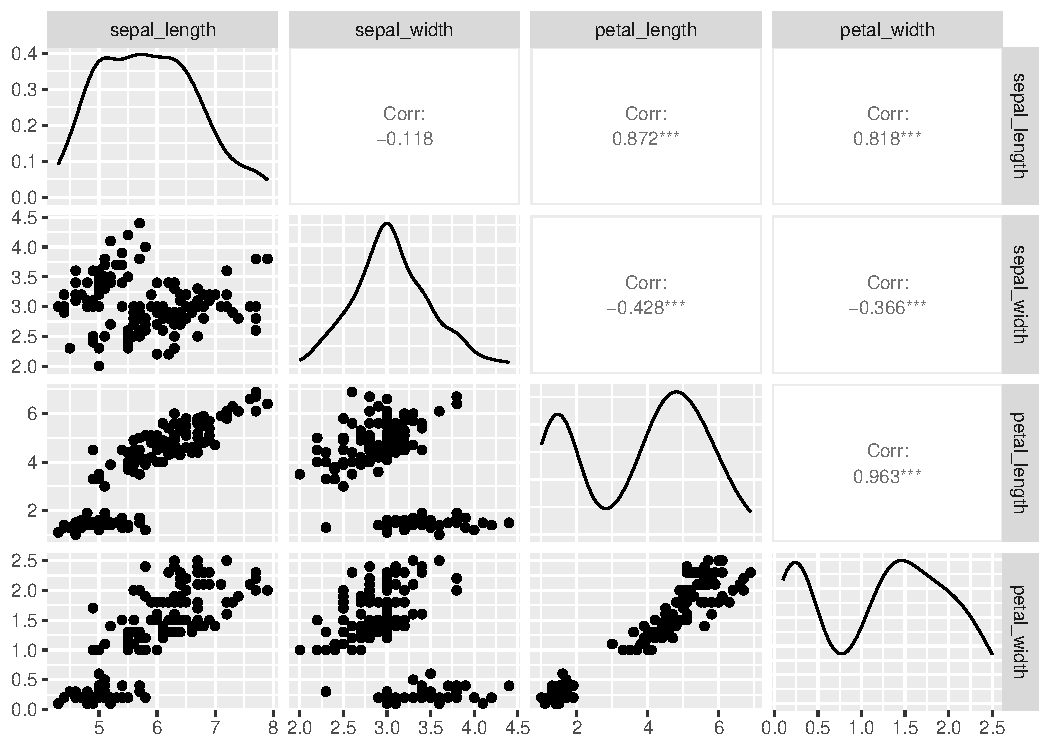
\includegraphics[keepaspectratio]{Análisis-exploratorios_files/figure-pdf/ggpairs-1.pdf}}

}

\caption{Matriz de dispersión y correlación de las variables
cuantitativas.}

\end{figure}%

La matriz de gráficos (scatterplots + histogramas + coeficientes de
correlación) permite evaluar de un vistazo correlaciones, distribuciones
marginales y relaciones lineales o no lineales entre variables.

\begin{itemize}
\item
  \textbf{Colinealidad fuerte}: \texttt{petal\_length} y
  \texttt{petal\_width} muestran correlación muy alta (r \textgreater{}
  0.9), lo que evidencia redundancia informativa.
\item
  \textbf{Correlaciones moderadas}: \texttt{sepal\_length} correlaciona
  de forma consistente con \texttt{petal\_length} (r ≈ 0.87), lo que
  sugiere que ambas crecen conjuntamente y pueden estar asociadas a un
  \textbf{gradiente de tamaño corporal general}.
\item
  \textbf{Menor asociación}: \texttt{sepal\_width} se muestra menos
  correlacionada con las demás, lo que indica que puede aportar
  información diferenciada en análisis multivariados.
\item
  \textbf{Separación por especie}: en las distribuciones univariadas y
  bivariadas se observa que las especies tienden a formar agrupamientos
  diferenciados, especialmente \texttt{setosa}, lo que sugiere potencial
  de clasificación/discriminación.
\item
  \textbf{Linealidad vs no linealidad}: las nubes de puntos muestran
  relaciones aproximadamente lineales, aunque con cierto solapamiento
  entre \emph{versicolor} y \emph{virginica}, lo cual podría requerir
  modelos más flexibles en análisis predictivos.
\item
  \textbf{Distribución}: Para \texttt{sepal\_length} es aproximadamente
  simétrica, con dispersión moderada. No aparecen valores extremos.
  \texttt{sepal\_width} presenta una dispersión menor que en
  \texttt{sepal\_length}; sin embargo, la distribución presenta cierta
  asimetría negativa (colas hacia valores pequeños). Finalmente tanto
  \texttt{petal\_length}como \texttt{petal\_width}muestran una
  distribución marcadamente bimodal, porque las especies difieren mucho
  en esta variable. Es la de mayor varianza relativa.
\end{itemize}

En presencia de \textbf{alta colinealidad} (r \textgreater{} 0.8),
considerar retener solo una variable del par altamente correlacionado si
el objetivo es simplificación. Emplear técnicas multivariadas (PCA,
análisis discriminante) para reducir dimensionalidad y evitar
inestabilidad en modelos de regresión.

\section{Distribución de variables morfométricas entre
especies}\label{distribuciuxf3n-de-variables-morfomuxe9tricas-entre-especies}

\begin{Shaded}
\begin{Highlighting}[numbers=left,,]
\CommentTok{\# Pasar el dataset a formato largo}
\NormalTok{iris\_long }\OtherTok{\textless{}{-}}\NormalTok{ df }\SpecialCharTok{\%\textgreater{}\%}
  \FunctionTok{pivot\_longer}\NormalTok{(}\AttributeTok{cols =} \SpecialCharTok{{-}}\NormalTok{species,}
               \AttributeTok{names\_to =} \StringTok{"Variable"}\NormalTok{,}
               \AttributeTok{values\_to =} \StringTok{"Valor"}\NormalTok{)}

\CommentTok{\# Gráfico unificado}
\FunctionTok{ggplot}\NormalTok{(iris\_long, }\FunctionTok{aes}\NormalTok{(}\AttributeTok{x =}\NormalTok{ species, }\AttributeTok{y =}\NormalTok{ Valor, }\AttributeTok{fill =}\NormalTok{ species)) }\SpecialCharTok{+}
  \FunctionTok{geom\_boxplot}\NormalTok{(}\AttributeTok{outlier.shape =} \DecValTok{21}\NormalTok{, }\AttributeTok{alpha =} \FloatTok{0.7}\NormalTok{) }\SpecialCharTok{+}
  \FunctionTok{facet\_wrap}\NormalTok{(}\SpecialCharTok{\textasciitilde{}}\NormalTok{ Variable, }\AttributeTok{scales =} \StringTok{"free\_y"}\NormalTok{) }\SpecialCharTok{+}
  \FunctionTok{labs}\NormalTok{(}
    \AttributeTok{title =} \StringTok{"Comparación de variables morfométricas en especies de Iris"}\NormalTok{,}
    \AttributeTok{x =} \StringTok{"Especies"}\NormalTok{,}
    \AttributeTok{y =} \StringTok{"Valor (cm)"}
\NormalTok{  ) }\SpecialCharTok{+}
  \FunctionTok{theme\_minimal}\NormalTok{(}\AttributeTok{base\_size =} \DecValTok{13}\NormalTok{) }\SpecialCharTok{+}
  \FunctionTok{theme}\NormalTok{(}
    \AttributeTok{plot.title =} \FunctionTok{element\_text}\NormalTok{(}\AttributeTok{hjust =} \FloatTok{0.5}\NormalTok{, }\AttributeTok{face =} \StringTok{"bold"}\NormalTok{),}
    \AttributeTok{legend.position =} \StringTok{"none"}\NormalTok{,}
    \AttributeTok{strip.text =} \FunctionTok{element\_text}\NormalTok{(}\AttributeTok{face =} \StringTok{"bold"}\NormalTok{)}
\NormalTok{  )}
\end{Highlighting}
\end{Shaded}

\begin{figure}[H]

{\centering \pandocbounded{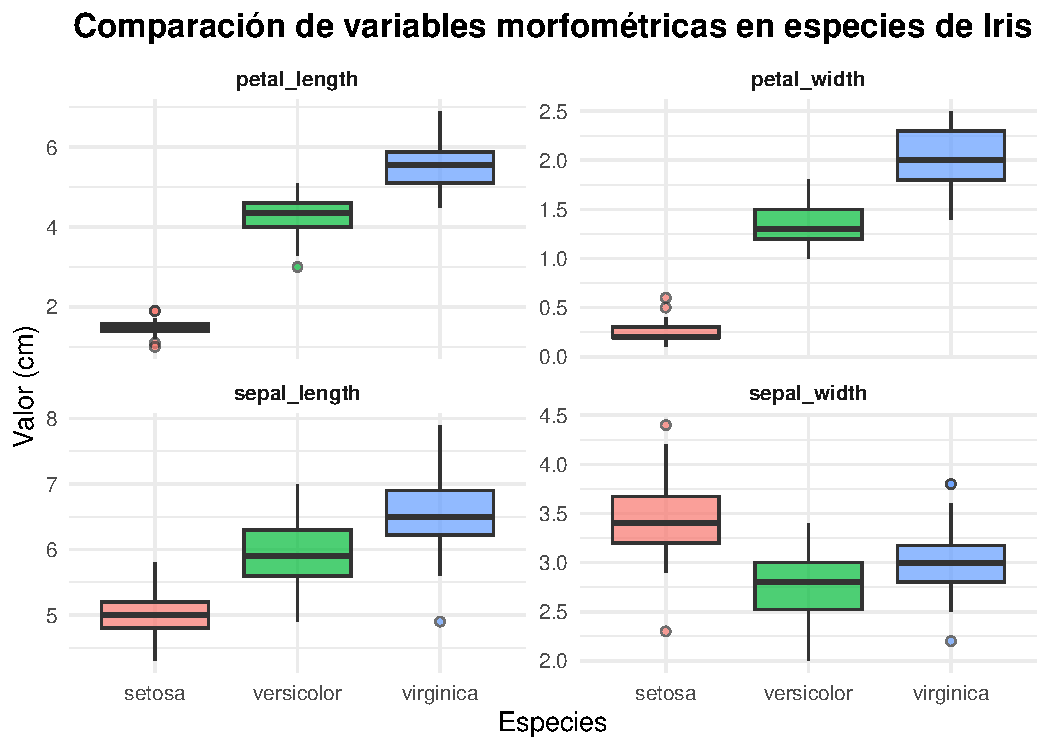
\includegraphics[keepaspectratio]{Análisis-exploratorios_files/figure-pdf/caja y bigotes-1.pdf}}

}

\caption{Distribución de variables morfométricas en tres especies de
Iris.}

\end{figure}%

En cuanto a la \textbf{longitud del sépalo (Sepal.Length)}, se observa
que \emph{Iris setosa} presenta los valores más bajos, con una mediana
cercana a los 5 cm, claramente diferenciada de las otras especies. Por
su parte, \emph{I. versicolor} e \emph{I. virginica} muestran longitudes
mayores y con bastante solapamiento, lo que dificulta separarlas
únicamente con esta variable. En consecuencia, Sepal.Length resulta útil
para discriminar a \emph{I. setosa}, pero limitado para distinguir entre
\emph{versicolor} y \emph{virginica}.

La \textbf{anchura del sépalo (Sepal.Width)} muestra distribuciones más
amplias y con solapamiento importante entre las tres especies. Aunque
\emph{setosa} tiende a tener sépalos ligeramente más anchos en promedio,
la alta variabilidad reduce su capacidad discriminante. Así, esta
variable por sí sola tiene bajo poder para diferenciar especies.

En el caso de la \textbf{longitud del pétalo (Petal.Length)}, se aprecia
una separación casi perfecta: \emph{setosa} forma un grupo completamente
aislado con valores mucho menores, mientras que \emph{versicolor} y
\emph{virginica} presentan medianas diferenciadas, aunque con cierto
solapamiento en sus rangos intercuartílicos. Esto convierte a
Petal.Length en una de las variables más informativas y clave para la
clasificación.

Finalmente, la \textbf{anchura del pétalo (Petal.Width)} también resulta
altamente discriminante. \emph{Setosa} presenta valores notablemente
bajos y sin superposición con las otras especies, mientras que
\emph{versicolor} y \emph{virginica} se diferencian con claridad, aunque
con menor margen que en el caso de Petal.Length. Esta variable se
perfila como una de las más robustas para separar especies,
especialmente en conjunto con Petal.Length.




\end{document}
